\section{Fixing Regularization and Evaluation of the model}

The model aims to perform well on all the tasks it has learned. To evaluate an estimator $\hat{x}$, we compare
its rank-one reconstruction $\hat{x}\hat{x}^T$ with the observations of each task.

\subsection{Evaluation Loss}\label{sec:eval}

\paragraph{Biased Evaluation Loss}
For given observations $Y_l = \lambda_l x_l x_l^T + Z_l \in \mathbb{R}^{n\times n}$, $l = 1,\dots,k$, and an
estimator $\hat{x} \in \mathbb{R}^n$ built from them, we define the Evaluation Loss as
\begin{equation}
  \mathcal{L}_{biased}(\hat{x}) := \sum_{l=1}^{k} \big\| Y_l - \hat{x}\hat{x}^T \big\|_F^2 .
  \label{eq:train_loss_def}
\end{equation}

Expanding the Frobenius norm, using $\|x_l\| = \|\hat{x}\| = 1$ and $x_l^T Z_l x_l \to 0$, the loss becomes in
the large $n$ limit
\begin{equation}
  \mathcal{L}_{biased}(\hat{x}) = \sum_{l=1}^{k} \Big[ -2\lambda_l\, m_l^2 \;-\; 2\,\varepsilon_l \Big] + \mathrm{cst},
  \qquad
  m_l := |\langle \hat{x}, x_l \rangle|, \quad
  \varepsilon_l := \hat{x}^T Z_l \hat{x}.
  \label{eq:train_loss}
\end{equation}
The full calculation is given in Appendix~\ref{an:exp-loss}.

\paragraph{The signal term.} The first term rewards the alignment of the estimator with each signal, weighted
by the strength $\lambda_l$ of that signal. This is the quantity we actually want to optimize.

\paragraph{The noise term and overfitting.} The second term shows that the loss decreases when the estimator is aligned with the noise $Z_l$. If $\hat{x}$ were
independent of $Z_l$, it would be delocalised on the eigenvectors of $Z_l$ and
$\varepsilon_l \to  0$. 

In other words, $\mathcal{L}_{biased}$ measures how well $\hat{x}\hat{x}^T$ reconstructs the
\emph{observations} (signal and noise), not the \emph{signals}. The estimator overfit the observation by fitting the noise. 

Minimizing
$\mathcal{L}_{\mathrm{eval-biased}}$ would therefore partly favour configurations in which the estimator fits the
noise, which is opposite to our goal of recovering $x_1, \dots, x_k$. 

\paragraph{Unbiased Evaluation Loss}
Let $Y'_l = \lambda_l x_l x_l^T + Z'_l$, $l = 1, \dots, k$, be new observations of the same signals, where
the $Z'_l$ are GOE matrices independent of the $Z_l$, and hence of $\hat{x}$. The test Evaluation Loss is
\begin{equation}
  \mathcal{L}_{\mathrm{eval}}(\hat{x}) := \sum_{l=1}^{k} \big\| Y'_l - \hat{x}\hat{x}^T \big\|_F^2 
\end{equation}

Since $\hat{x}$ is independent of $Z'_l$, $\hat{x}^T Z'_l \hat{x} \to 0$ and the noise term disappears:
\begin{equation}
  \boxed{ \; \mathcal{L}_{\mathrm{eval}}(\hat{x}) = -2 \sum_{l=1}^{k} \lambda_l\, m_l^2 + \mathrm{cst}. \; }
    \label{eq:test_loss}
\end{equation}
A good estimator is then one that maximizes its overlaps with the signals, weighted by their strengths. The
difference between both losses,
\begin{equation}
  \mathcal{L}_{biased} - \mathcal{L}_{eval} = 2 \sum_{l=1}^{k} \varepsilon_l \;\geq\; 0,
\end{equation}
 quantifies how much of the apparent performance on the training data
comes from fitting the noise. The full expression of the noise terms $\varepsilon_l$ for naive method and method A are presented in Appendix \ref{an:Naive-Loss} and \ref{an:A_full_Loss}.




\subsection{Fixing the hyperparameters $\alpha$ and $\mu_R$}
\label{sec:optimal_param}

Each method has    hyperparameter that sets the balance between the two tasks: the importance factor $\alpha$ for the naive method, and the regularisation strength $\mu_R$ for Methods A and B. We fix it such that the estimator learns both tasks as well as possible, i.e.\ such that it minimises the test Evaluation Loss of Eq.~\eqref{eq:test_loss}. Writing $t \in \{\alpha, \mu_R\}$ for the hyperparameter of the method under study, the only terms of $\mathcal L_{\mathrm{eval}}$ that depend on $t$ are the overlaps $m_l(t)$ of the estimator with the signals, so that
\begin{equation}
    t^* = \operatorname*{arg\,min}_{t}\ \mathcal L_{\mathrm{eval}}(t)
    = \operatorname*{arg\,max}_{t}\ \sum_{l=1}^{k}\lambda_l\, m_l(t)^2 .
    \label{eq:t_opt}
\end{equation}
When the optimum lies inside the admissible range ($0 < \alpha^* < 1$ or $0 < \mu_R^* < \infty$), it satisfies the stationarity condition
\begin{equation}
    \frac{\partial\mathcal L_{\mathrm{eval}}}{\partial t}(t^*)
    = -2\sum_{l=1}^{k}\lambda_l\,\frac{\partial\, m_l^2}{\partial t}(t^*) = 0 .
    \label{eq:mu_opt}
\end{equation}
The optimum may also lie at a boundary, for instance $\alpha^* \in \{0, 1\}$ when the two tasks are weakly correlated and mixing them dilutes the signal below the detection threshold. In that case, Eq.~\eqref{eq:mu_opt} does not hold, and Eq.~\eqref{eq:t_opt} must be used directly. The overlaps are given in closed form by Eq.~\eqref{eq:overlap_naive} for the naive method, by Eq.~\eqref{eq:overlap_A} for Method A, and by Eqs.~\eqref{eq:B_norm}--\eqref{eq:B_overlap} for Method B. Equation~\eqref{eq:mu_opt} is therefore a scalar equation, which we solve numerically.

\paragraph{Numerical results.} Figure~\ref{fig:loss_opt} shows the Evaluation Losses of the three methods as functions of their hyperparameter, for $\lambda_1 = 3$, $\lambda_2 = 2$ and $\rho = 0.5$. We draw four observations from it.
\begin{itemize}
    \item \textbf{Theory and simulations agree.} The theoretical test loss $-2\sum_l\lambda_l m_l^2$ matches both the overlaps measured in simulations and the loss evaluated on fresh observations $\rdmmat Y'_l$ with independent noise. The theoretical biased loss of Appendix~\ref{an:Naive-Loss} (naive method) and Appendix~\ref{an:A_full_Loss} (Method A) matches its simulated counterpart. The biased loss of Method B is only shown numerically.

    \item \textbf{The biased loss is optimistic and shifts the optimum.} The biased loss lies about $2$ below the test loss for all three methods. This gap is the generalisation gap $2\sum_l\varepsilon_l$ of Section~\ref{sec:eval}: part of the apparent performance on the training data comes from fitting the noise. The gap is not constant, so it also moves the optimum. Minimising the biased loss would give $\alpha^* \simeq 0.71$ instead of $0.81$, $\mu_R^* \simeq 0.42$ instead of $0.48$ for Method A, and $\mu_R^* \simeq 0.18$ instead of $0.23$ for Method B, i.e.\ systematically less weight on the first task.

    \item \textbf{The optimum is a non-trivial trade-off.} For $\alpha \to 0$ or $\mu_R \to 0$, the estimator is the top eigenvector of $\rdmmat Y_2$, with $m_2^2 = 1 - \lambda_2^{-2}$ and $m_1^2 = \rho^2 m_2^2$: the loss tends to $-2\big(\lambda_1\rho^2 + \lambda_2\big)(1-\lambda_2^{-2}) \simeq -4.1$ (catastrophic forgetting). For $\alpha \to 1$ or $\mu_R \to \infty$, the estimator is $\hat{\vect x}^{(1)}$, with $m_1^2 = 1 - \lambda_1^{-2}$ and $m_2^2 = \rho^2 m_1^2$: the loss tends to $-2\big(\lambda_1 + \lambda_2\rho^2\big)(1-\lambda_1^{-2}) \simeq -6.2$ (no learning of task~$2$). At the optimum, the loss reaches about $-6.7$.

    \item \textbf{The sequential methods match the naive method.} At their optimum, Methods A and B reach a test loss of about $-6.70$, slightly below the $-6.65$ of the naive method, although the naive method sees both observations at the same time. A possible explanation is that the sequential methods only keep the rank-one projection of the first task, $\Lambda\,\hat{\vect x}^{(1)}\hat{\vect x}^{(1)\top}$, and thus discard the bulk noise $\rdmmat Z_1$, whereas the naive method keeps the noise of both observations. The values of $\mu_R^*$ for Methods A and B are not directly comparable, since $\mu_R$ weights different penalties in the two methods.
\end{itemize}

\begin{figure}[t]
    \centering
    \begin{subfigure}[t]{0.32\textwidth}
        \centering
        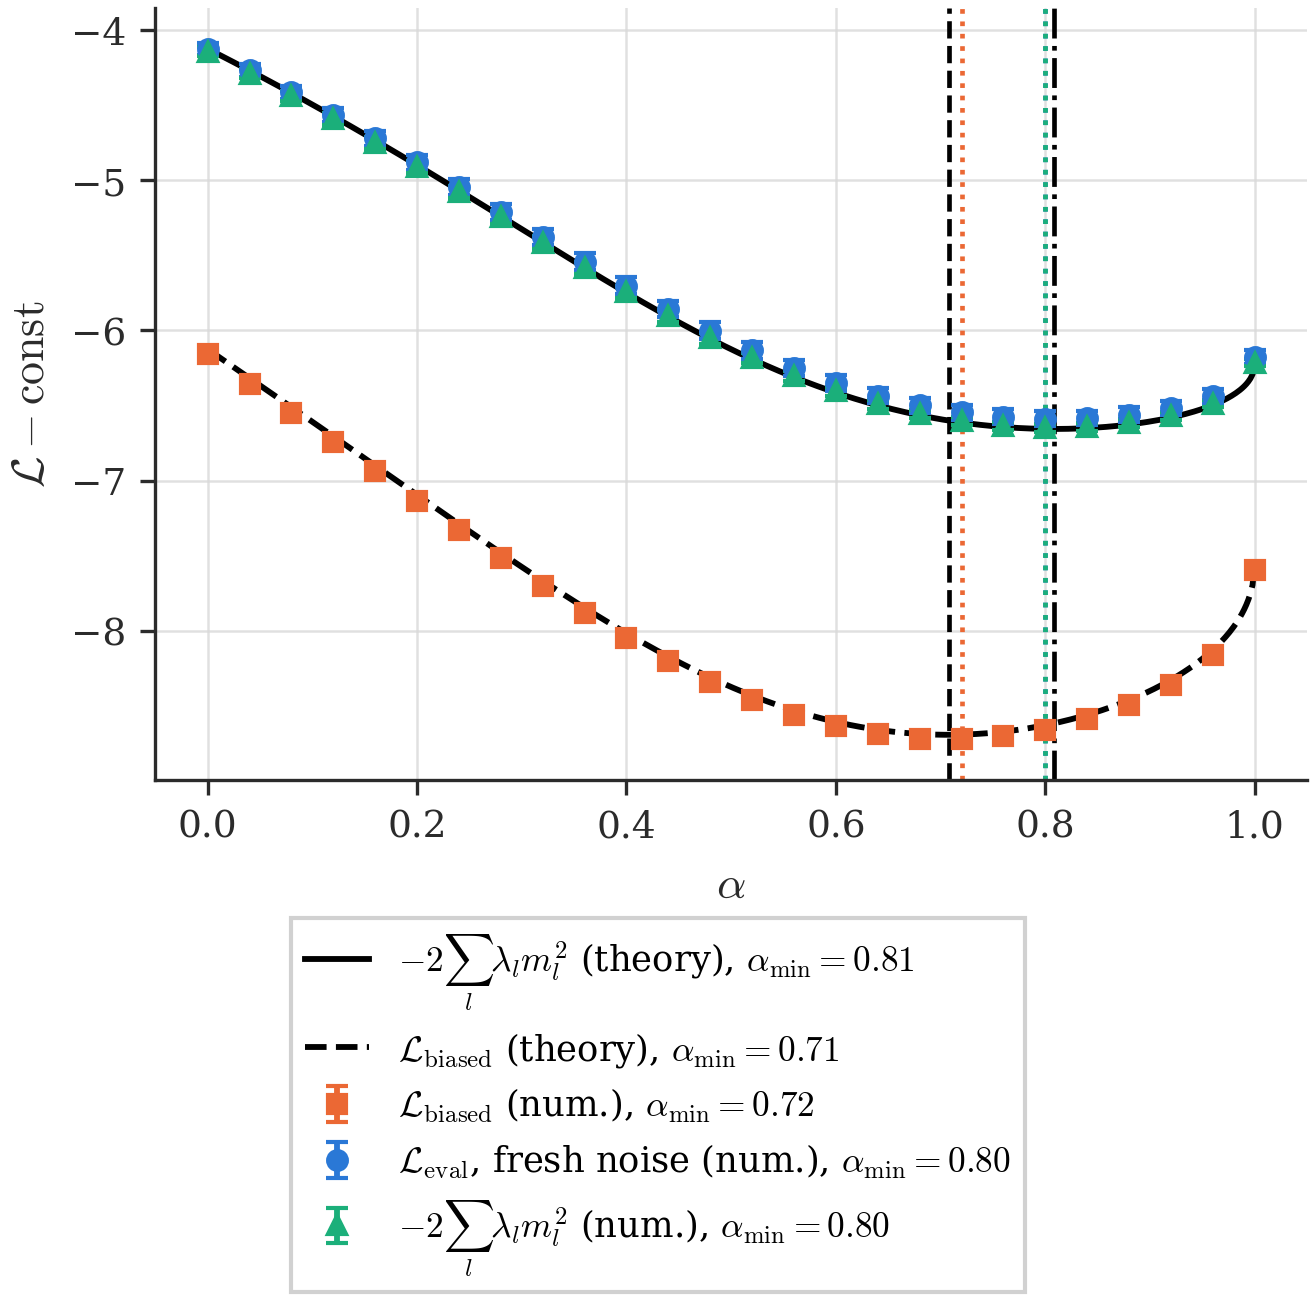
\includegraphics[width=\linewidth]{figures/loss_study/loss_biased_naive_vs_alpha_lam1=3.0_lam2=2.0_rho=0.5_report.png}
        \caption{Naive method, as a function of $\alpha$.}
        \label{fig:loss_opt_naive}
    \end{subfigure}\hfill
    \begin{subfigure}[t]{0.32\textwidth}
        \centering
        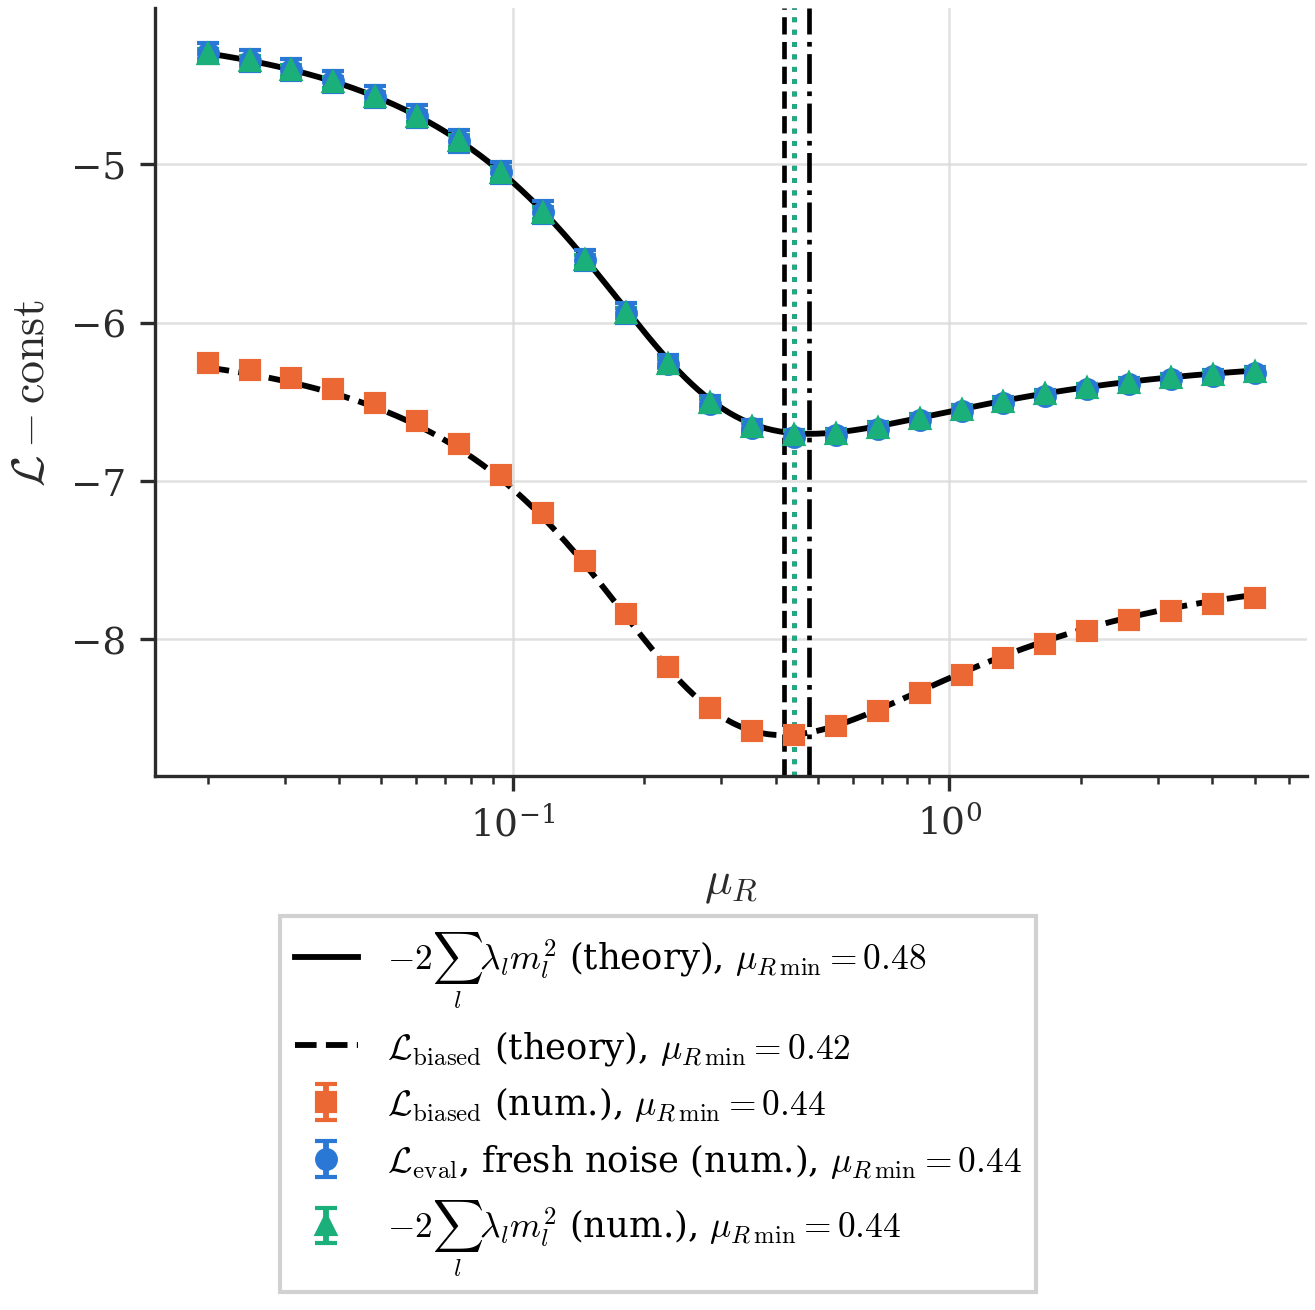
\includegraphics[width=\linewidth]{figures/loss_study/loss_biased_A_vs_mu_lam1=3.0_lam2=2.0_rho=0.5_report.png}
        \caption{Method A, as a function of $\mu_R$.}
        \label{fig:loss_opt_A}
    \end{subfigure}\hfill
    \begin{subfigure}[t]{0.32\textwidth}
        \centering
        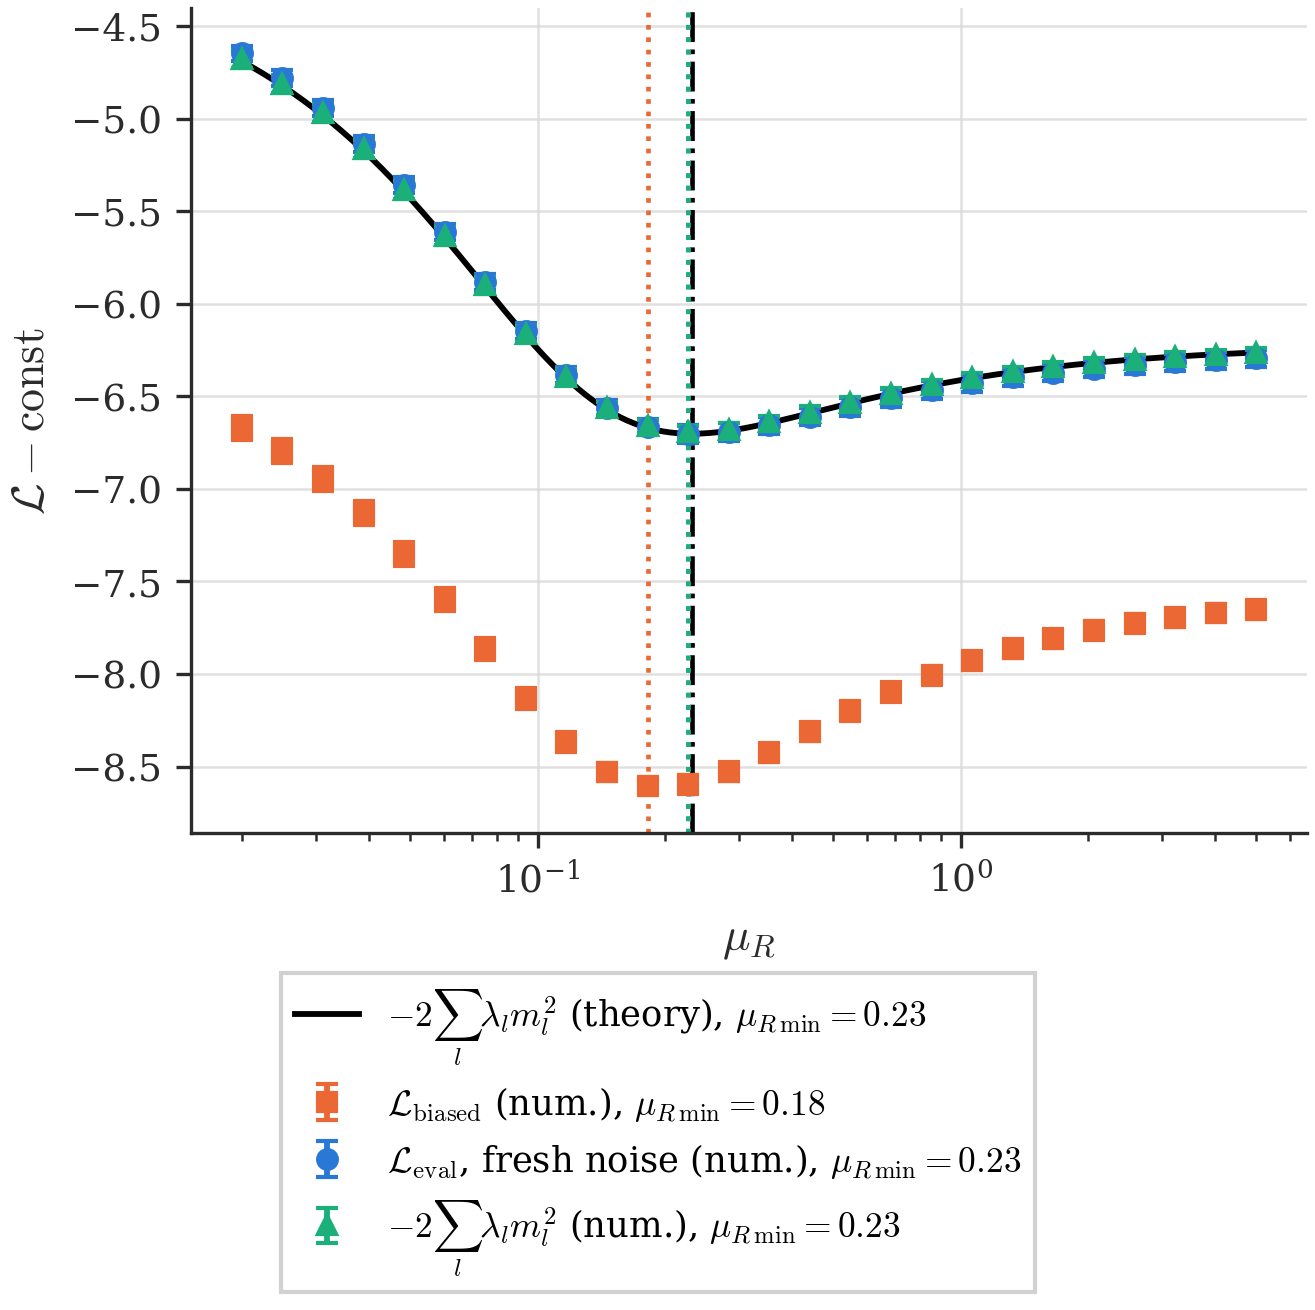
\includegraphics[width=\linewidth]{figures/loss_study/loss_biased_B_vs_mu_lam1=3.0_lam2=2.0_rho=0.5_report.png}
        \caption{Method B, as a function of $\mu_R$.}
        \label{fig:loss_opt_B}
    \end{subfigure}
    \caption{Evaluation Losses (up to a constant) as functions of the hyperparameter of each method, for $\lambda_1 = 3$, $\lambda_2 = 2$ and $\rho = 0.5$. Solid line: theoretical test loss $-2\sum_l\lambda_l m_l^2$. Dashed line: theoretical biased loss. Symbols: simulations with $n = \dots$, averaged over $\dots$ realisations (error bars: standard deviation), for the biased loss (squares), the loss evaluated on fresh noise (circles) and $-2\sum_l\lambda_l m_l^2$ computed from the measured overlaps (triangles). Vertical lines: minimisers of each curve, whose values are given in the legends. The theoretical biased loss of Method B is not computed.}
    \label{fig:loss_opt}
\end{figure}


\subsection{Comparison methods}
\begin{figure}[H]
    \centering
    \begin{subfigure}[t]{0.5\textwidth}
        \centering
        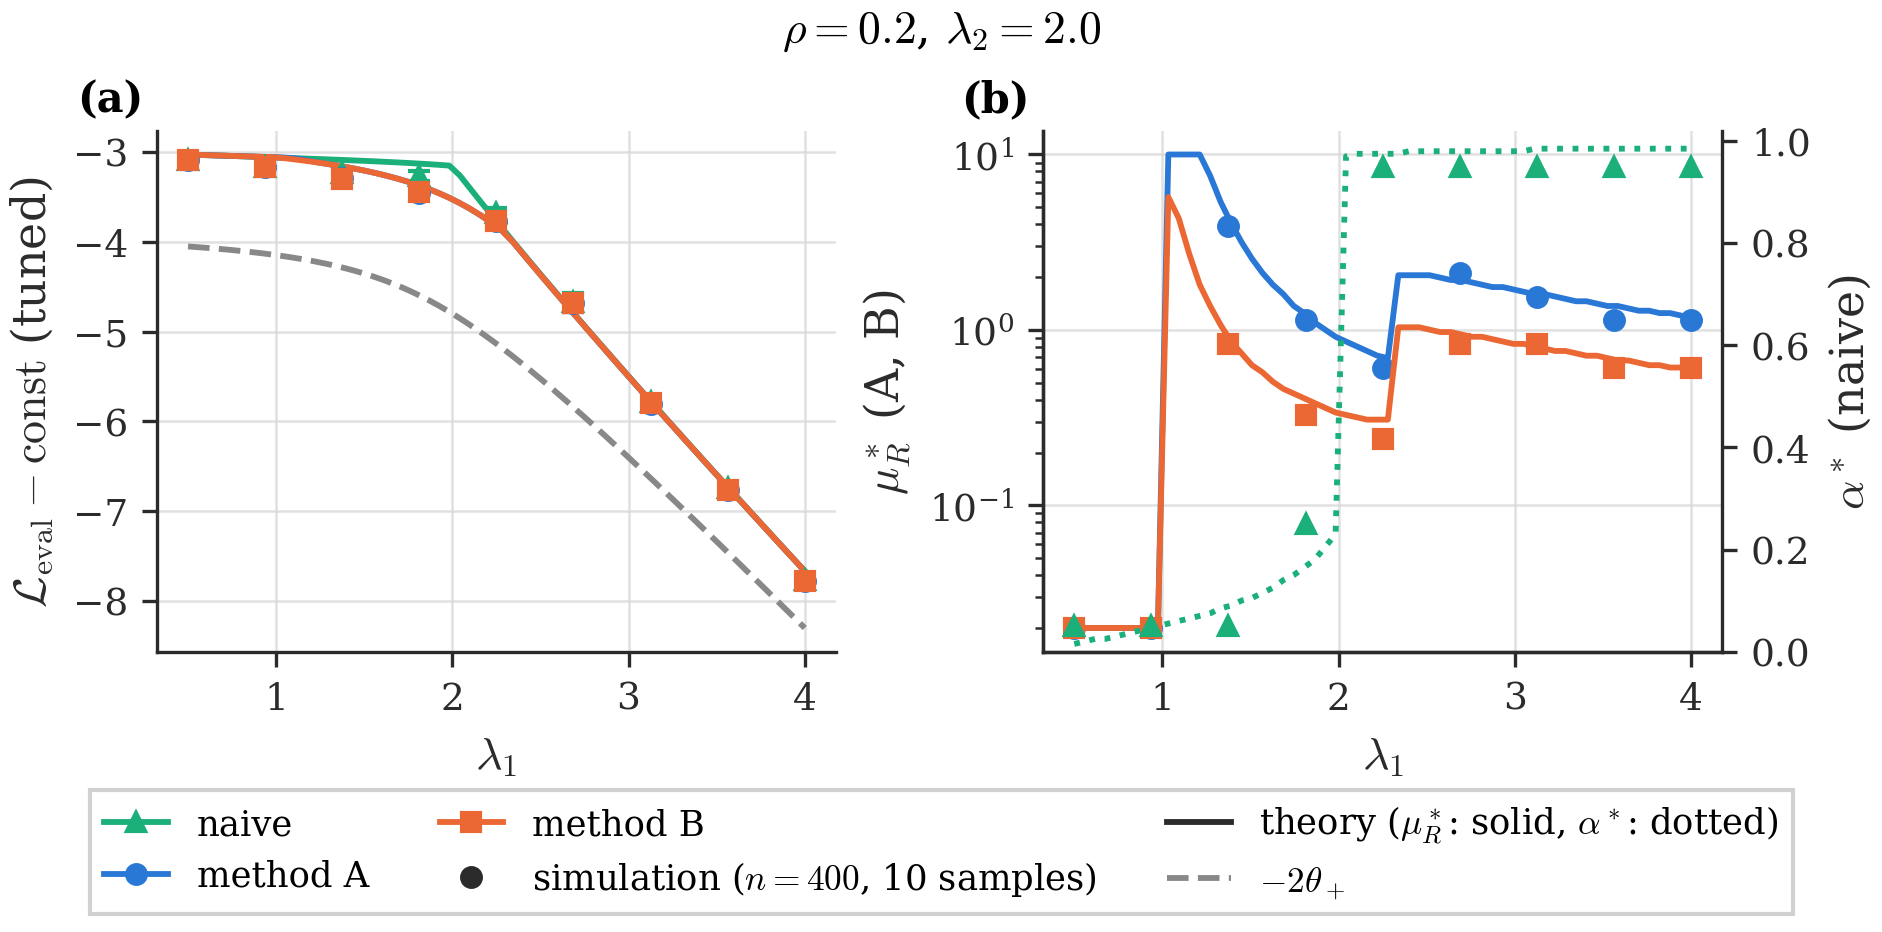
\includegraphics[width=\linewidth]{figures/loss_study/loss_unbiased_tuned_vs_lam1_lam2=2.0_rho=0.2_n=400_report.png}
        \caption{Naive method, as a function of $\alpha$.}
        \label{fig:loss_opt_naive}
    \end{subfigure}\hfill
    \begin{subfigure}[t]{0.5\textwidth}
        \centering
        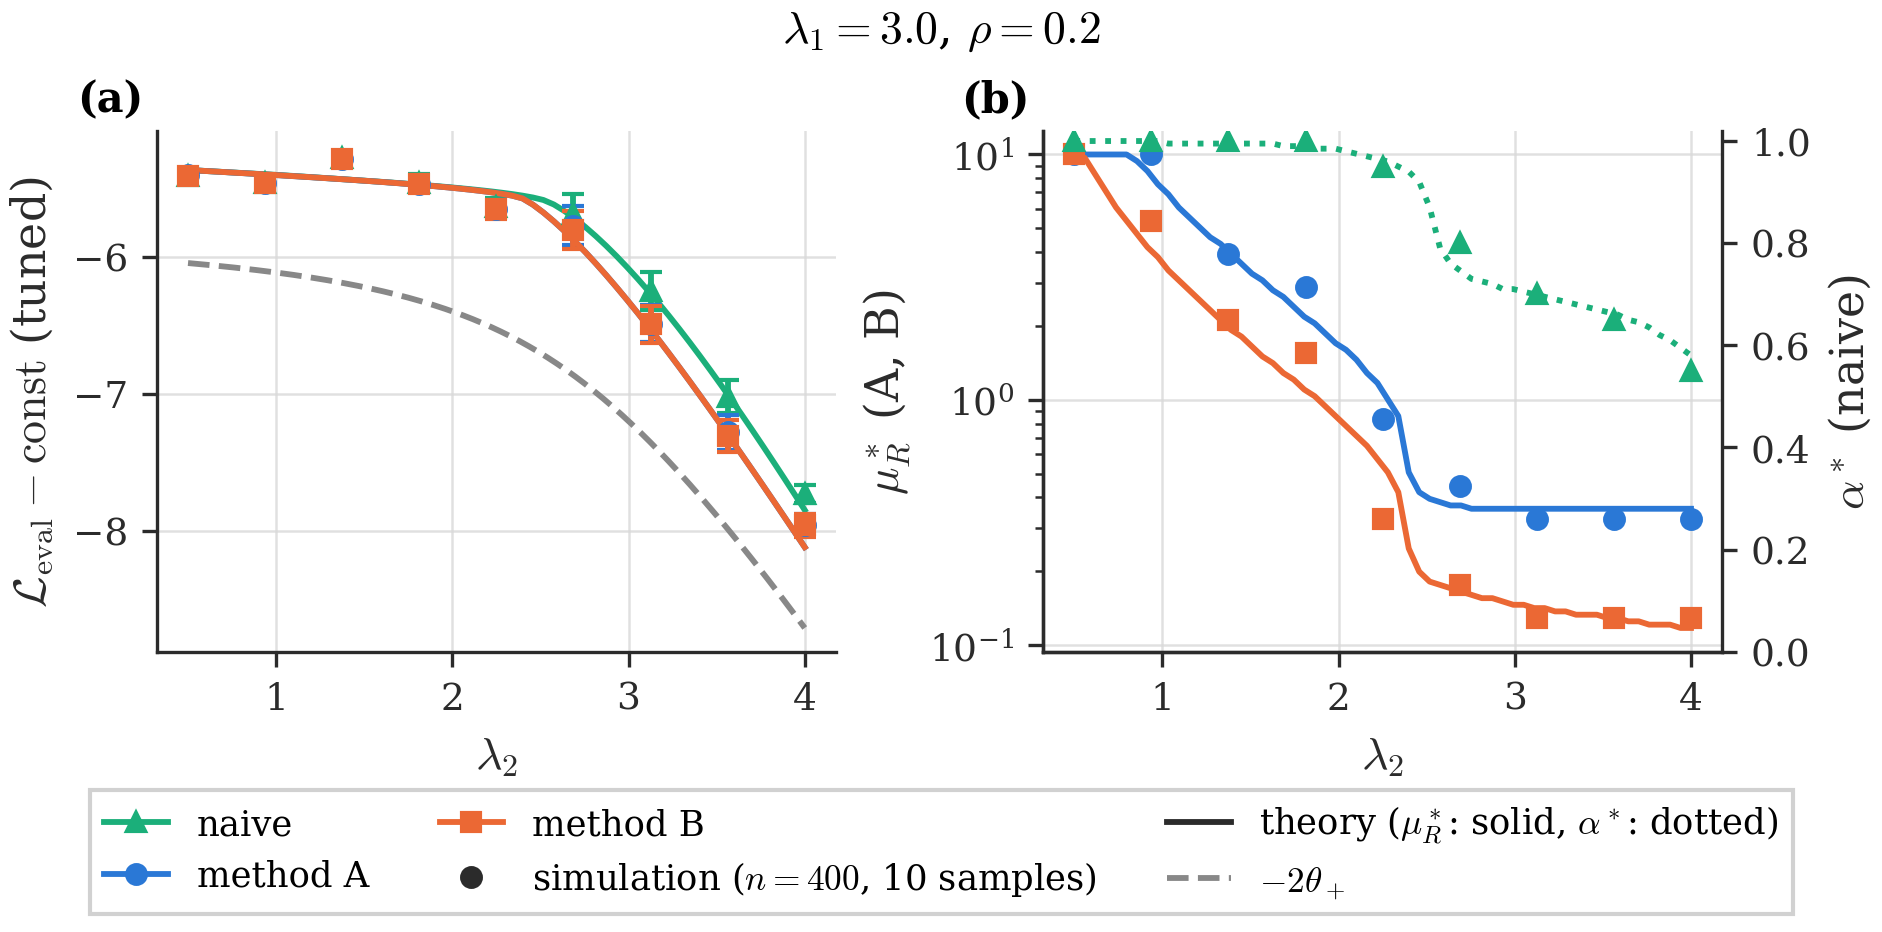
\includegraphics[width=\linewidth]{figures/loss_study/loss_unbiased_tuned_vs_lam2_lam1=3.0_rho=0.2_n=400_report.png}
        \caption{Method A, as a function of $\mu_R$.}
        \label{fig:loss_opt_A}
    \end{subfigure}\hfill
    \begin{subfigure}[t]{0.5\textwidth}
        \centering
        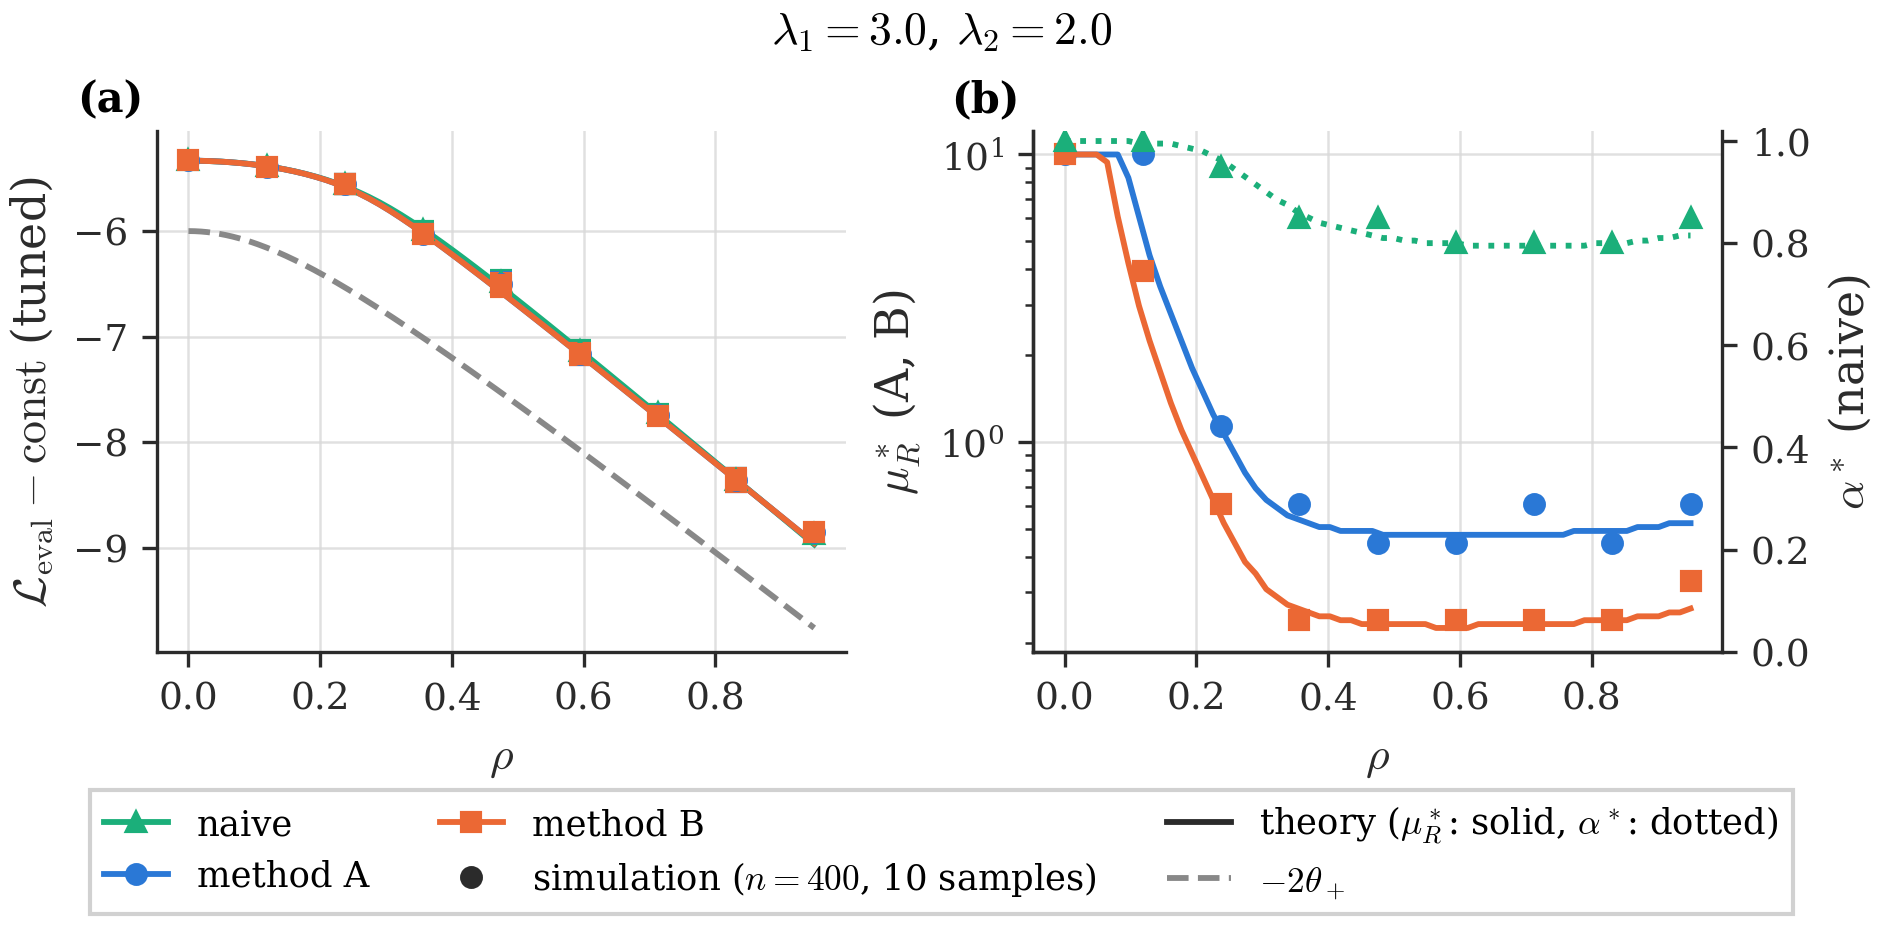
\includegraphics[width=\linewidth]{figures/loss_study/loss_unbiased_tuned_vs_rho_lam1=3.0_lam2=2.0_n=400_report.png}
        \caption{Method B, as a function of $\mu_R$.}
        \label{fig:loss_opt_B}
    \end{subfigure}
    \caption{}
    \label{fig:loss_opt}
\end{figure}
,
\begin{figure}[H]
    \centering
    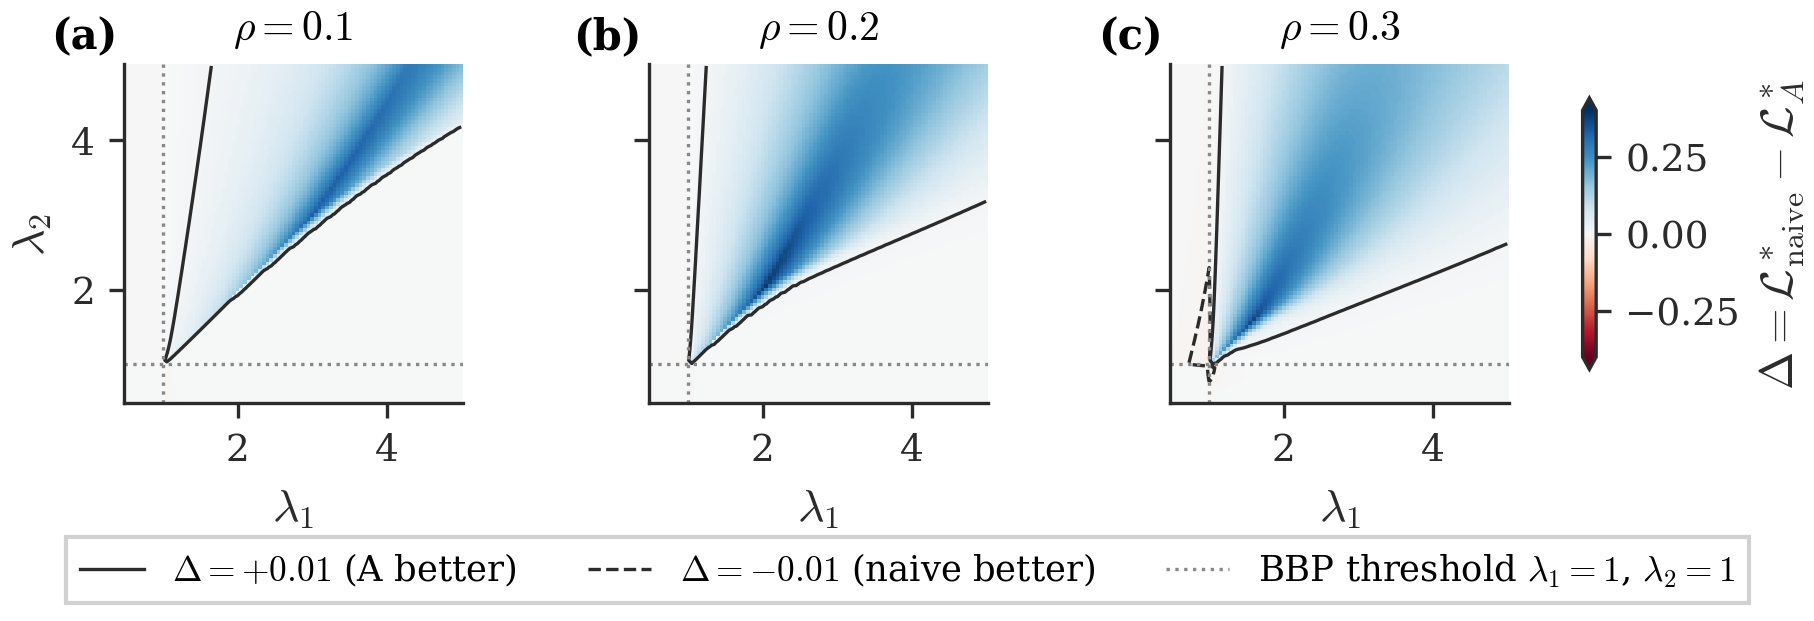
\includegraphics[width=0.9\linewidth]{figures/loss_study/heatmap_gap_naive_A_rho=0.1_0.2_0.3_report.png}
    \caption{Caption}
    \label{fig:placeholder}
\end{figure}
,
\begin{figure}[H]
    \centering
    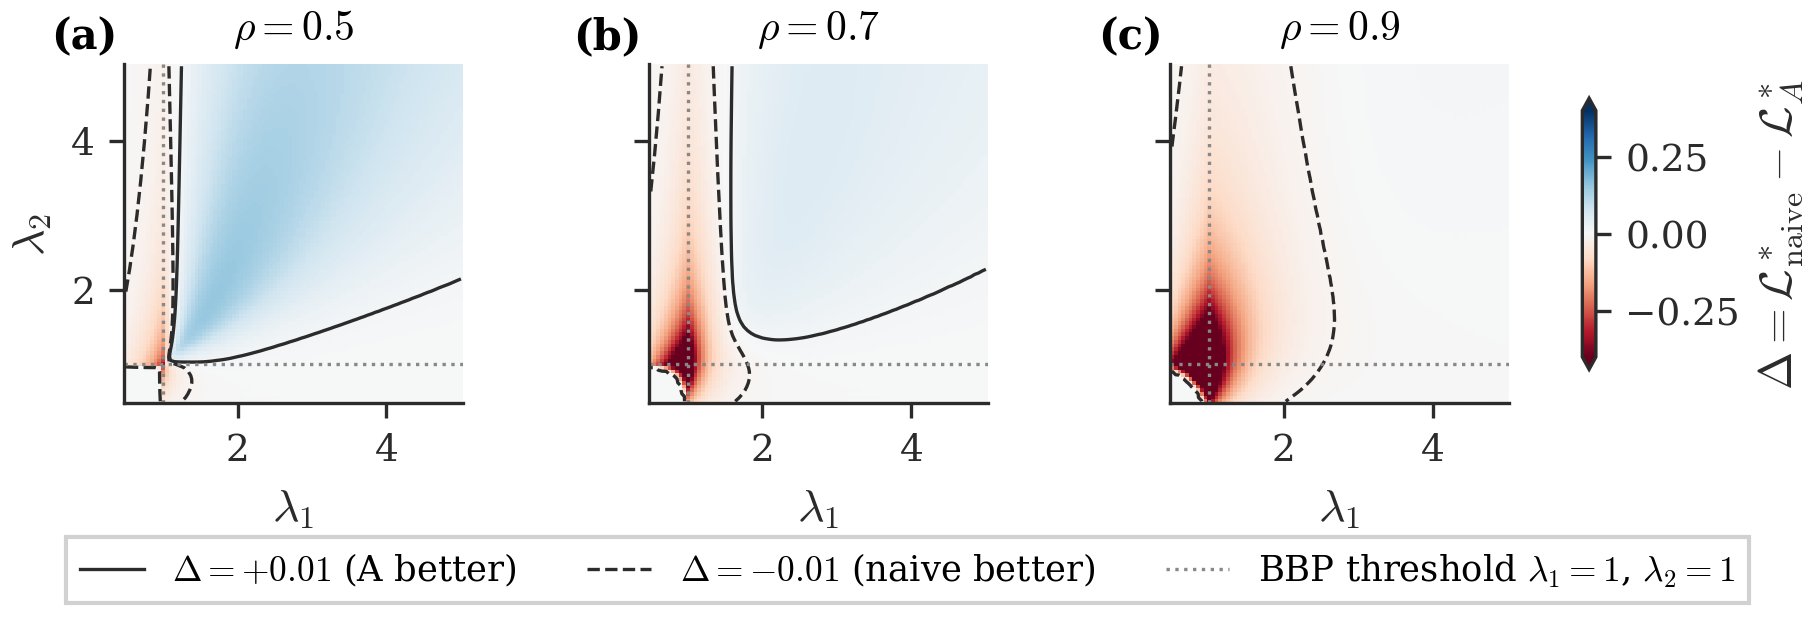
\includegraphics[width=0.9\linewidth]{figures/loss_study/heatmap_gap_naive_A_rho=0.5_0.7_0.9_report.png}
    \caption{Caption}
    \label{fig:placeholder}
\end{figure}
\begin{comment}
\subsubsection{Methode A: Optimal parameter}
Lets consider the method A estimator of our signals $\vect \hat x _A \equiv \vect \hat x _A(\mu_R) $. 

The condition eq.\ref{eq:mu_opt} on optimal regularization parameter $\mu_R^*$ is then:

\begin{equation}
    \boxed{
-4\left(\frac{\partial\vect{\hat x}_A(\mu_R^*)}{\partial\mu_R}\right)^T
\left(
\rdmmat Y_1+\rdmmat Y_2
-2\rdmmat I_n
\right)\vect{\hat x}_A (\mu_R^*) = 0.
}
\end{equation}

Let us consider the Method~A estimator, $\hat{\vect x}_A\equiv\hat{\vect x}_A(\mu_R)$ and consider the unormalized estimator $\Tilde{\vect x}_A$.

The optimality condition is therefore:
\[
\boxed{
\big(\partial \mu_R\Tilde{\vect x}_A\big)^{\,T}
\left[
Y-\frac{
\Tilde{\vect x}_A^{\,T}Y\Tilde{\vect x}_A
}{
\Tilde{\vect x}_A^{\,T}\Tilde{\vect x}_A
}
\rdmmat I_3
\right]
\Tilde{\vect x}_A=0.
}
\]

where $\vect v_{\max}$, $\widetilde{\vect v}$ and $\partial_{\mu_R}\widetilde{\vect v} = \frac{\partial \vect \Tilde v}{\partial \mu_R}$
are given in the paragraph \ref{sec:v_max_methodeA}.
The derivation of this condition is given in Annexe \ref{an:mu_rcond}.

\end{comment}


